
\begin{figure*}[!ht]
  \begin{center}
  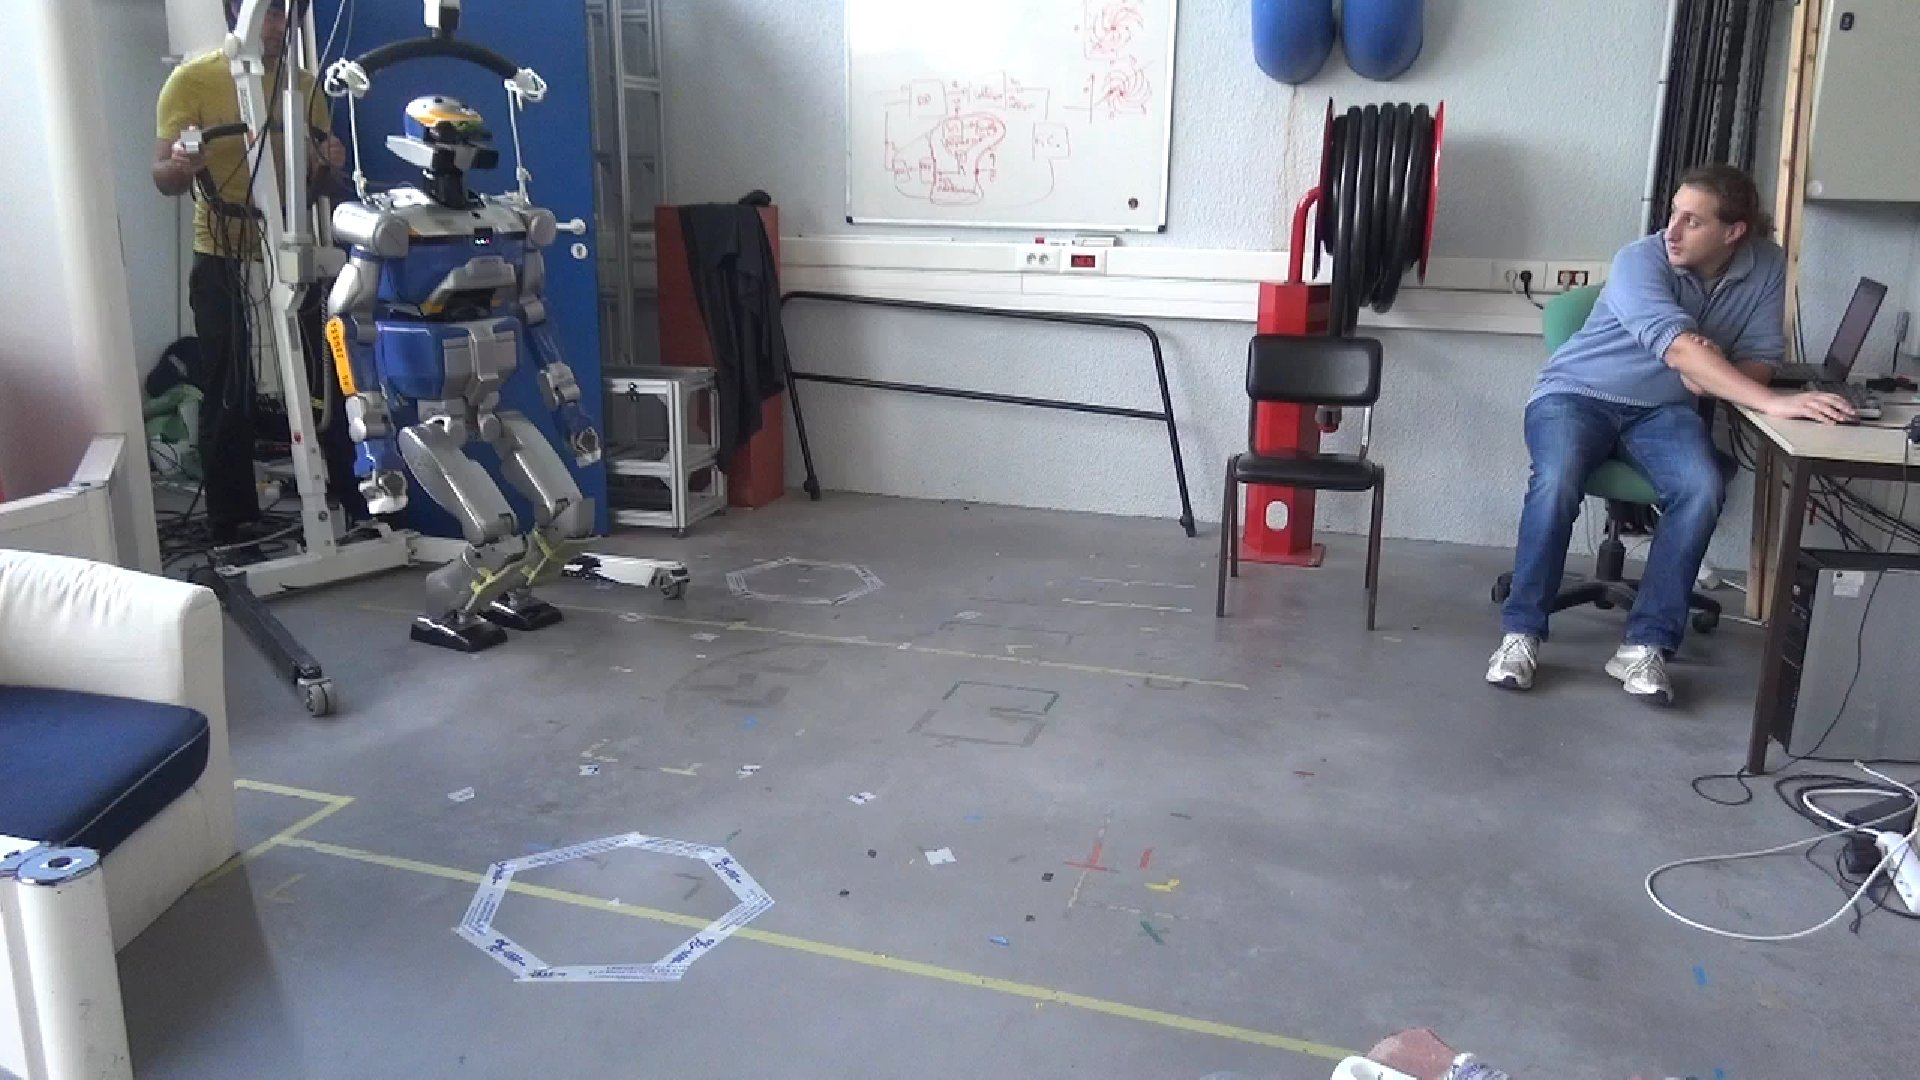
\includegraphics[trim={7.0cm 0.0cm 20.0cm 0.0cm}, clip, width=0.2\widthValue]
    {./fig/fastwalk1.jpeg}
  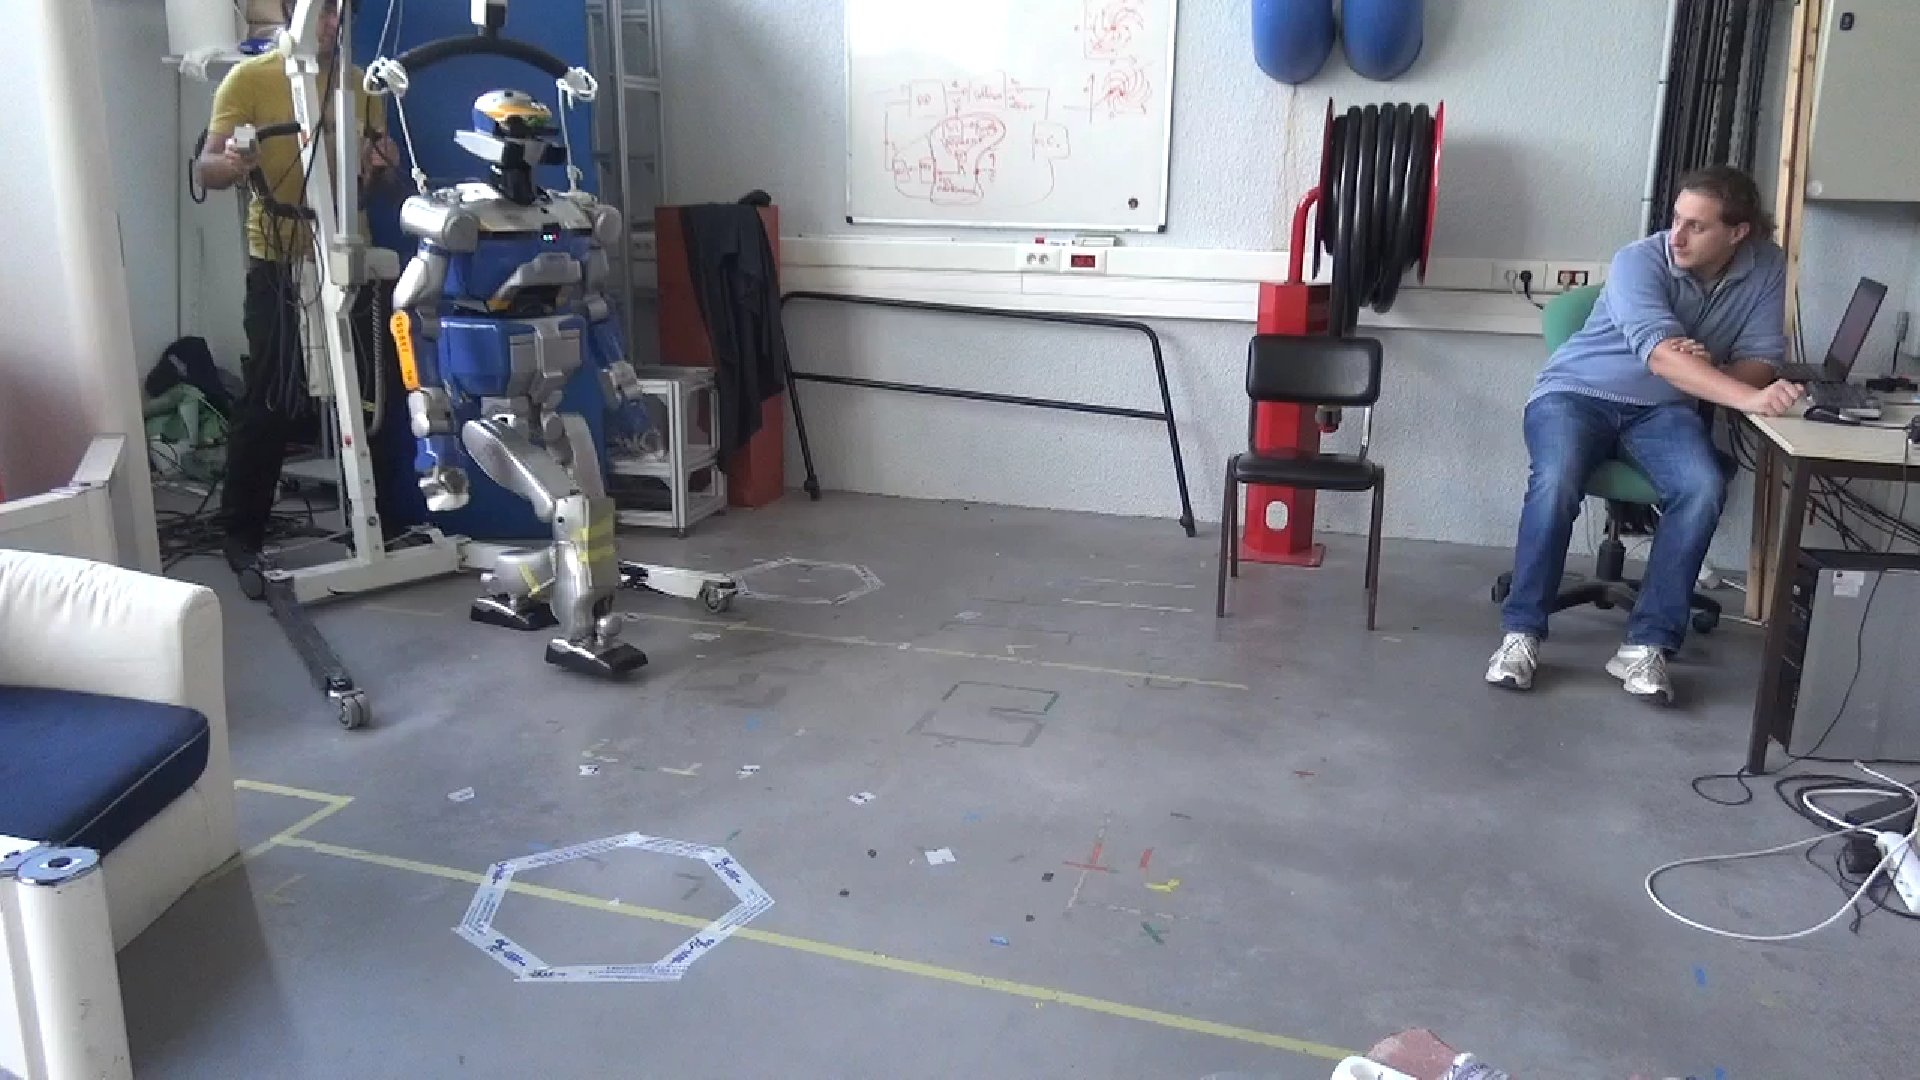
\includegraphics[trim={7.0cm 0.0cm 20.0cm 0.0cm}, clip, width=0.2\widthValue]
    {./fig/fastwalk2.jpeg}
  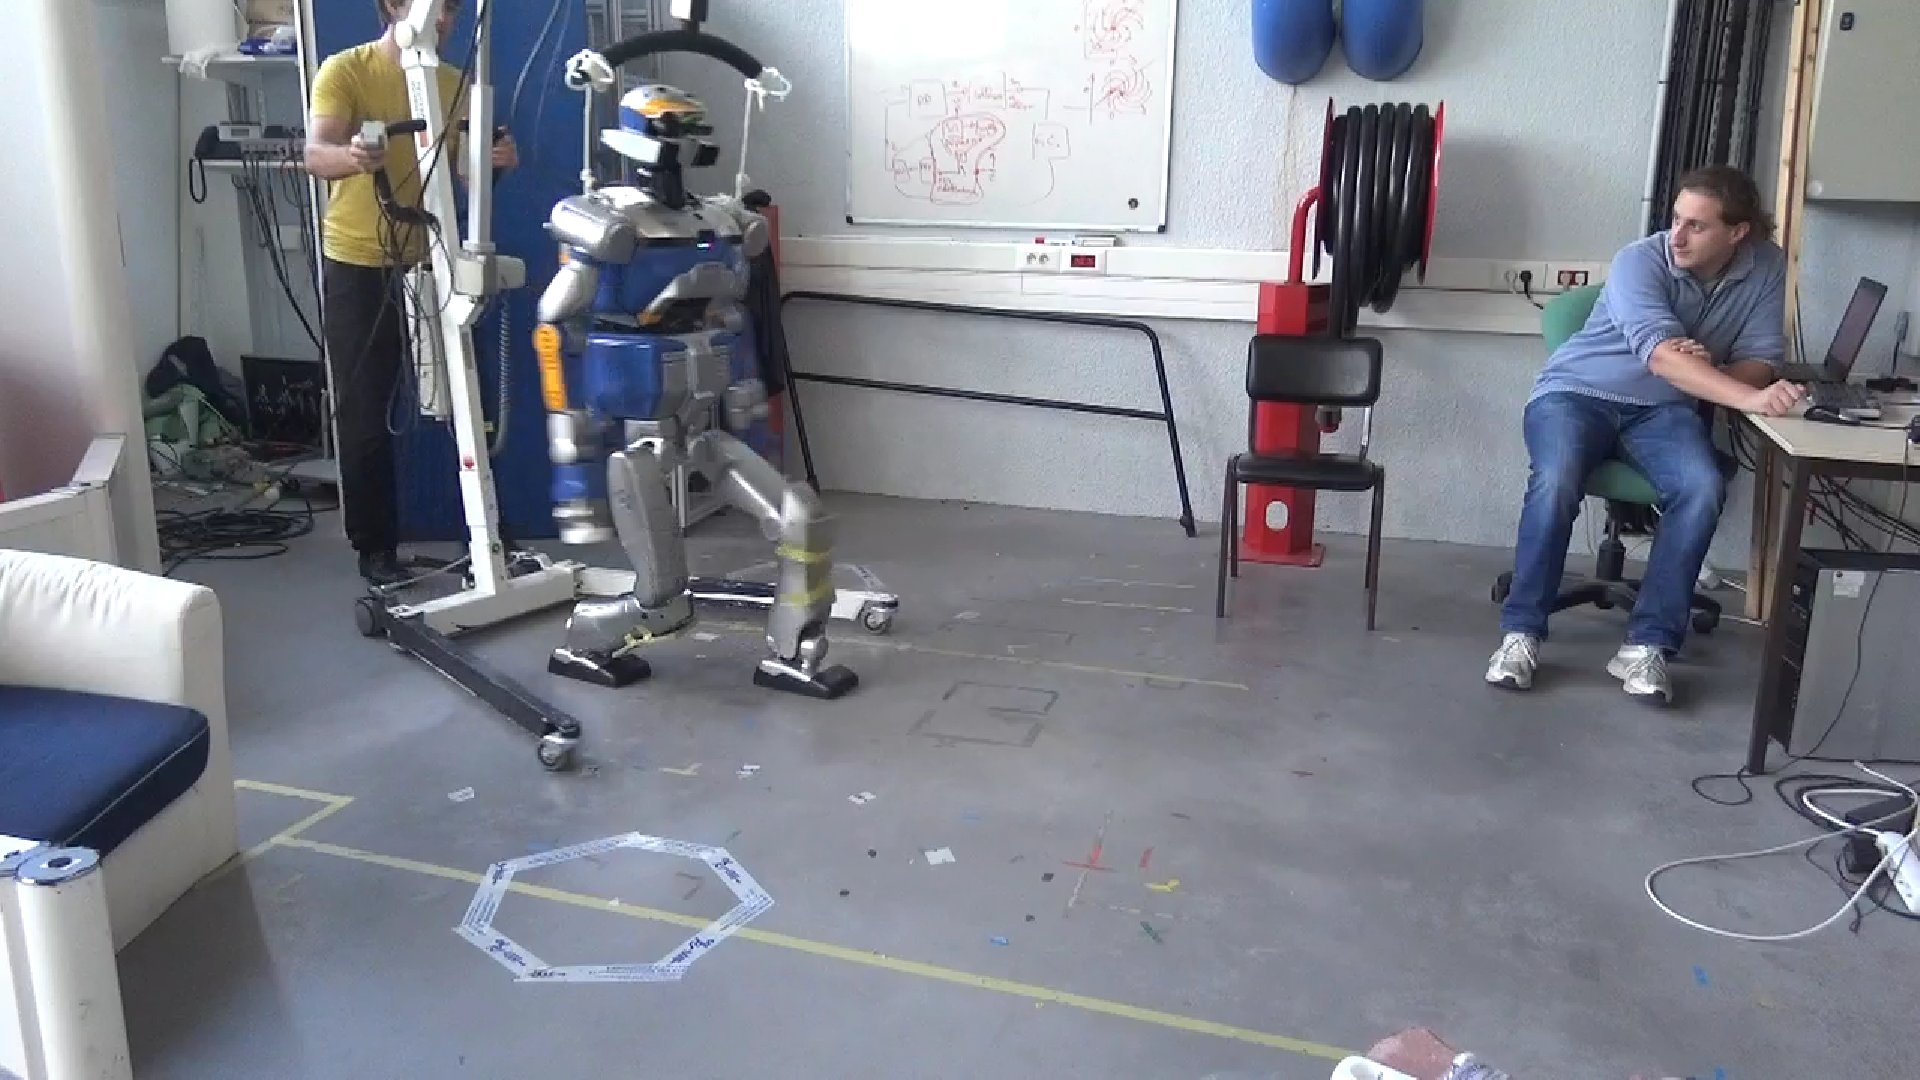
\includegraphics[trim={7.0cm 0.0cm 20.0cm 0.0cm}, clip, width=0.2\widthValue]
    {./fig/fastwalk3.jpeg}
  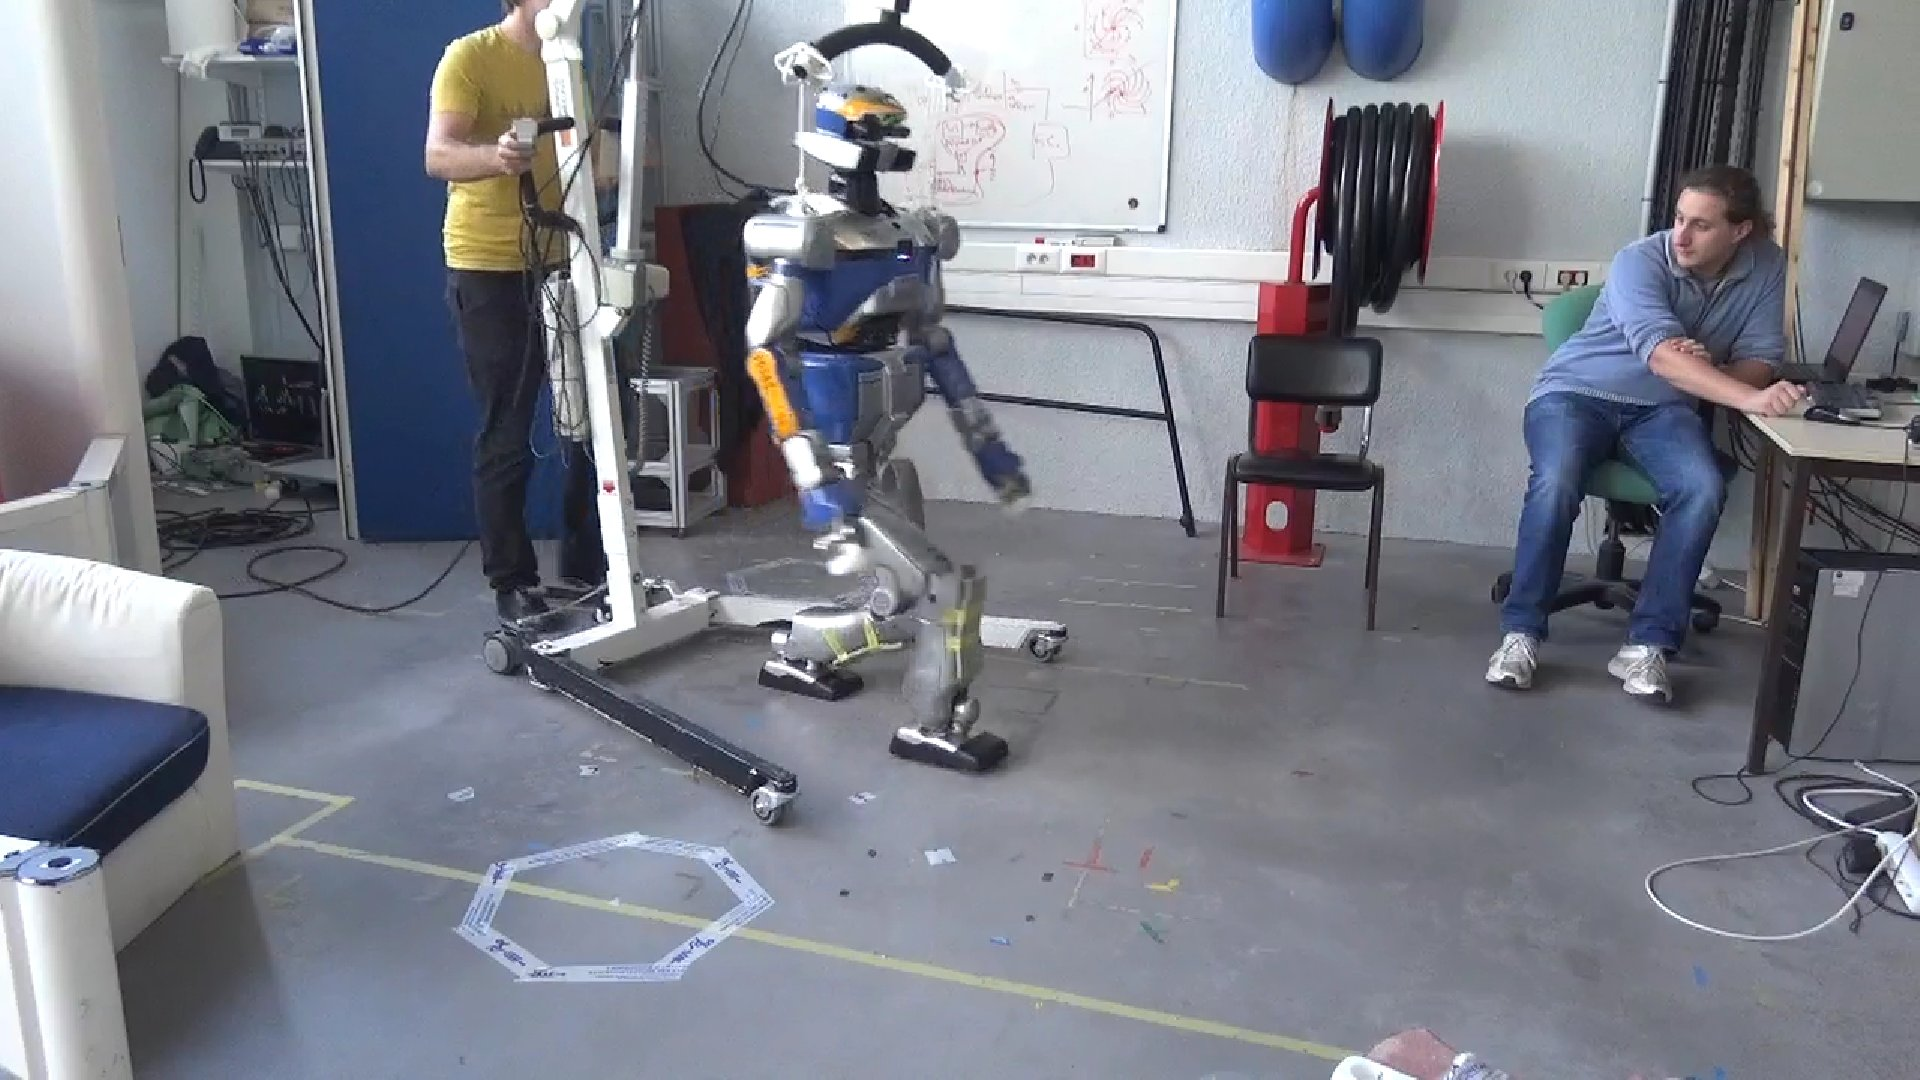
\includegraphics[trim={7.0cm 0.0cm 20.0cm 0.0cm}, clip, width=0.2\widthValue]
    {./fig/fastwalk4.jpeg}
  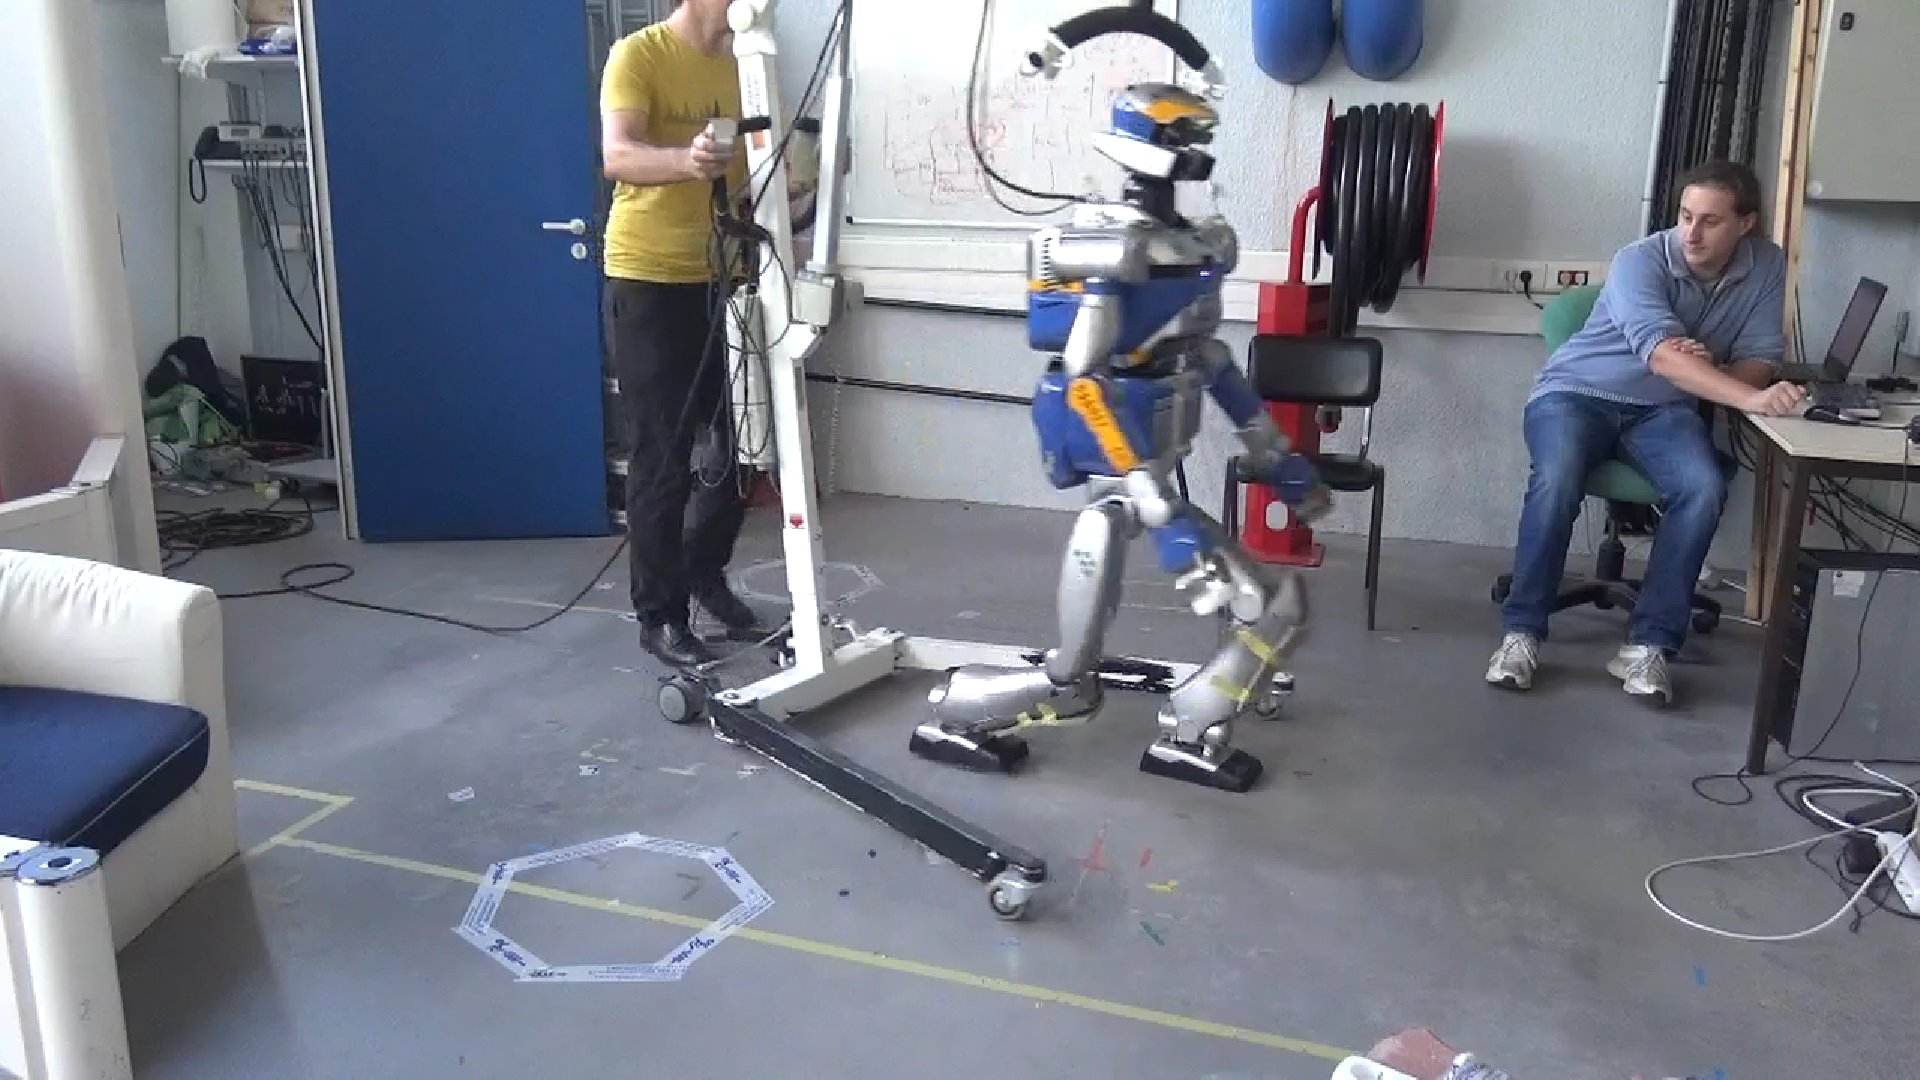
\includegraphics[trim={18.0cm 0.0cm 10.0cm 0.0cm}, clip, width=0.2\widthValue]
    {./fig/fastwalk5.jpeg}
  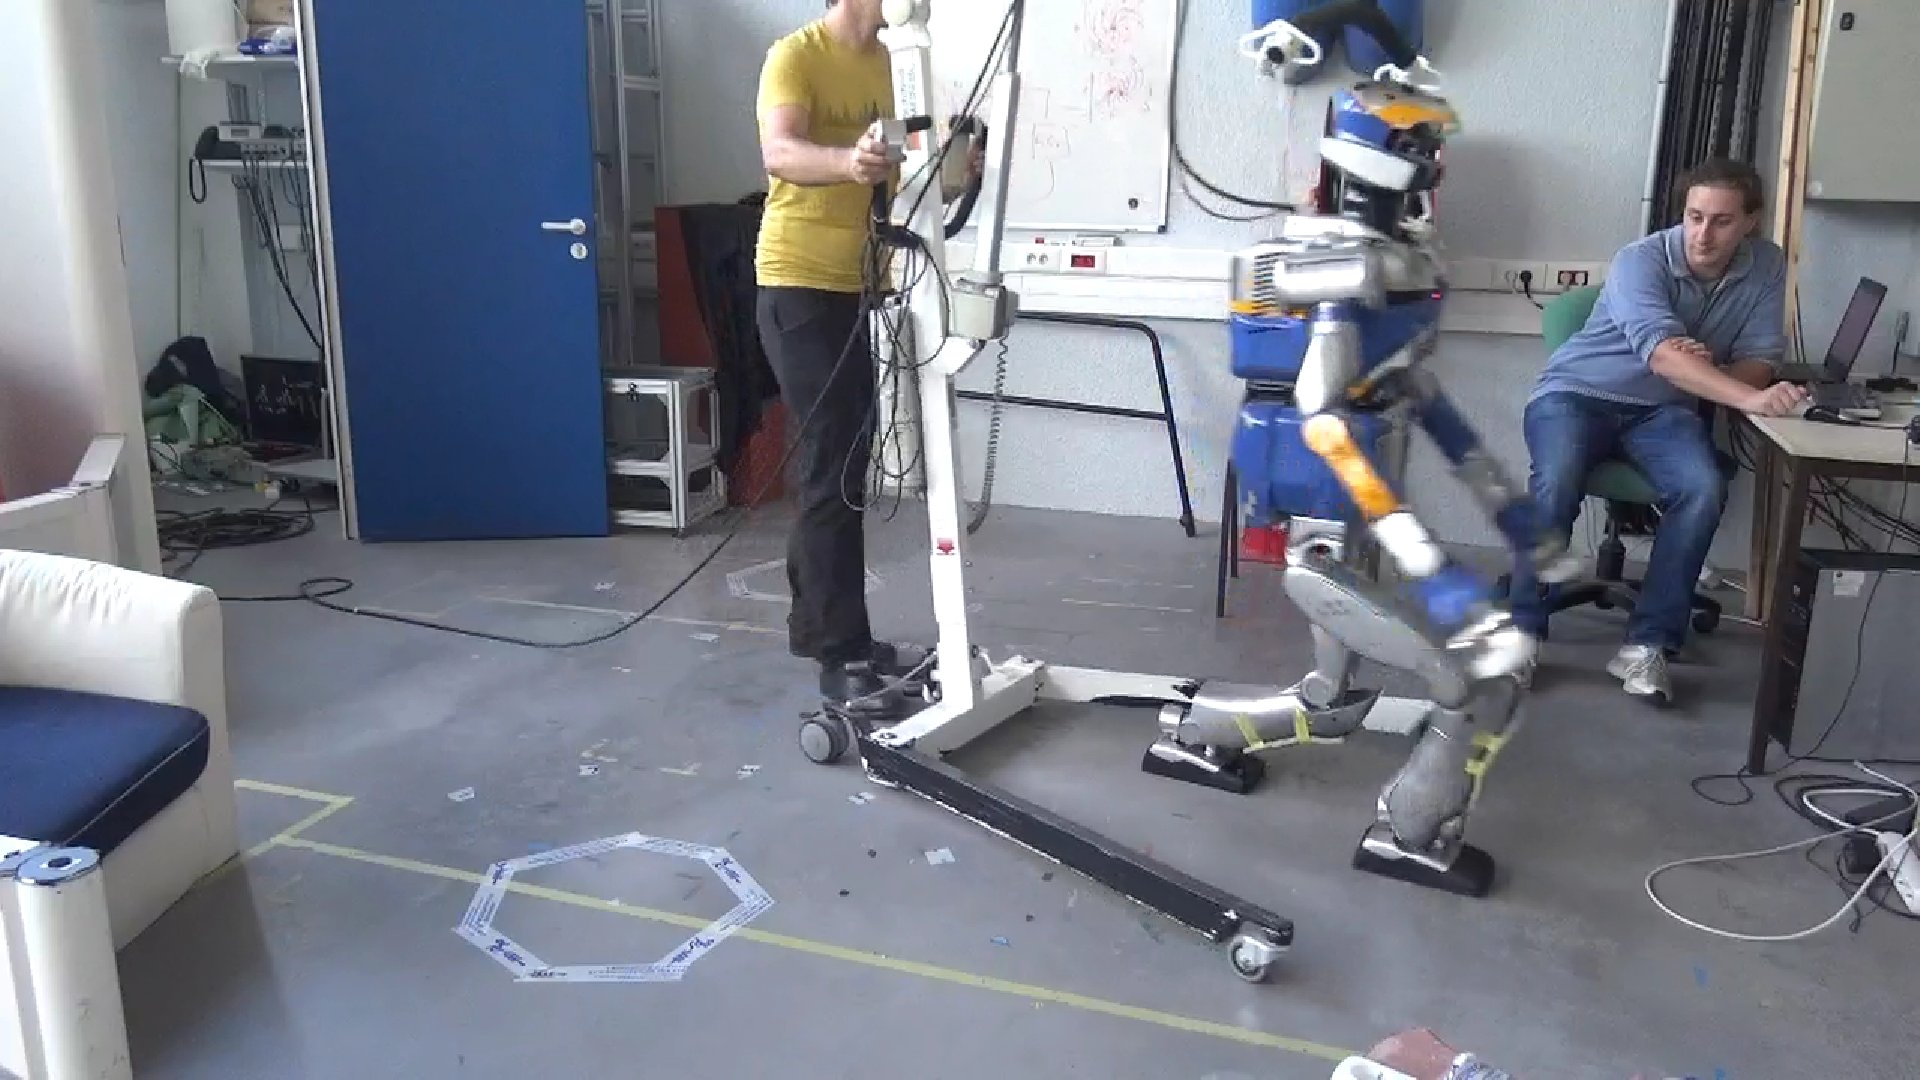
\includegraphics[trim={23.0cm 0.0cm 5.0cm 0.0cm}, clip, width=0.2\widthValue]
    {./fig/fastwalk6.jpeg}
  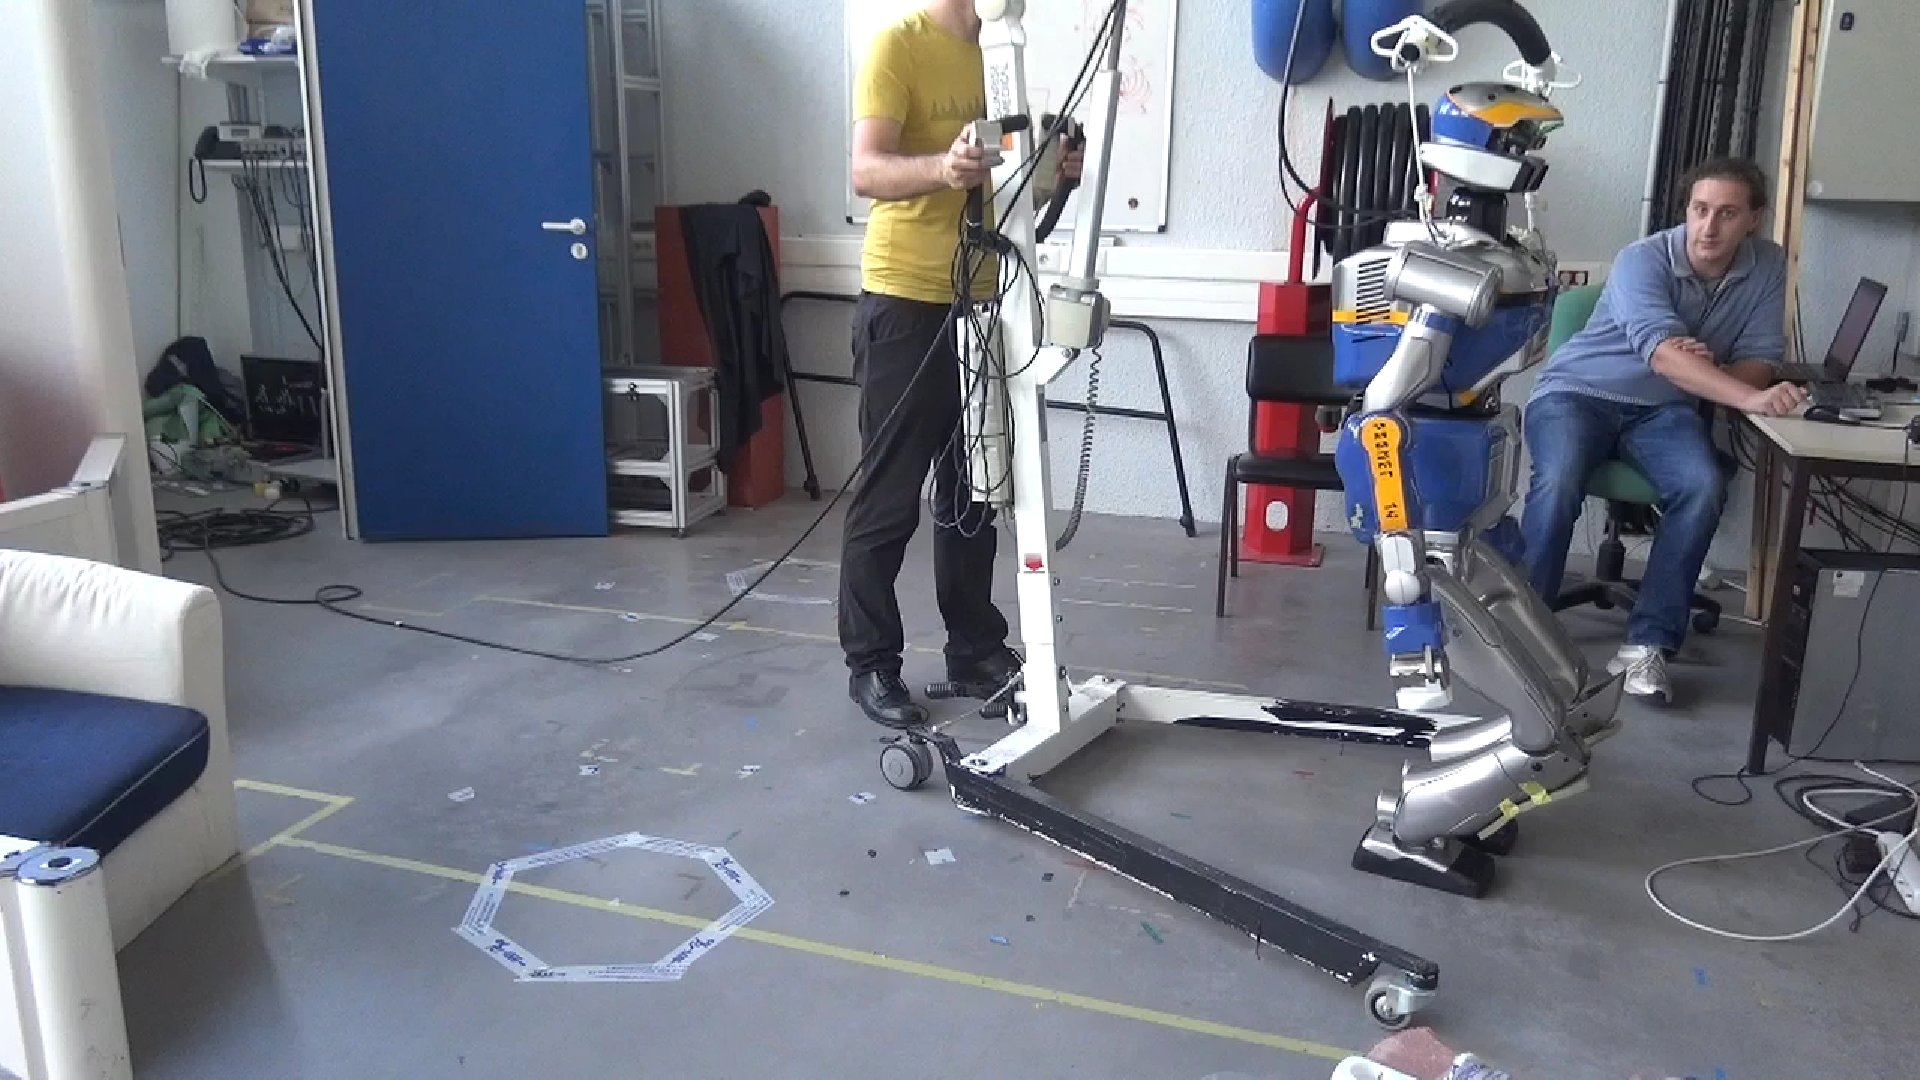
\includegraphics[trim={23.0cm 0.0cm 5.0cm 0.0cm}, clip, width=0.2\widthValue]
    {./fig/fastwalk7.jpeg}
  \caption{
    Experiment 1: Walking in straight line with enjambment of $100$cm.
  }
  \label{fig:moviepicture}
  \end{center}
\end{figure*}

\section{Experimental Results}
\label{sec:experimental}


Two main experiments carried out on the HRP-2 robot are presented. The first experiment concerns the generation of a classic walking motion: it is a unitary test but it is important to properly understand the behavior of our solver compared to classical walking pattern generators. The second experiment is the climbing stairs scenario depicted in Fig. \ref{fig:moviepicture}, where the robot has to make use of the handrail to help its ascension of the stairs. We additionally show two movements of running and standing up, that were not executed by the robot but help to demonstrate the versatility of the approach.

\subsection{Experimental setup}
All the computations (contact planning and WPG) were performed offline on a Intel Xeon(R) CPU E3-1240 v3 @ 3.40GHz. The contact planner is open-source and is available at \url{https://github.com/humanoid-path-planner}. The OCP is solved using the proprietary software MUSCOD provided by the Interdisciplinary Center for Scientific Computing (IWR) of Heidelberg University. This software offers a OCP toolkit (e.g. integration and numerical-differentiation routines) along with an efficient sparse sequential-quadratic-program solver.
The whole-body trajectory is obtained from the contact sequence and the COM and angular-momentum trajectory using a second-order inverse kinematics (i.e. computes the joint acceleration using the jacobian pseudoinverse). The typical tasks where the tracking of the contact placements, the tracking of the COM position and an additional posture task to keep the configuration close to the planned postures.
The computed trajectories are then executed by the real robot. For the walking experiments, we used a closed-loop control provided with the robot (called the stabilizer) to stabilize the movements of the rubber bush inside each foot~\cite{6942670}. The stabilizer was not used for climbing the stairs, because it is not able to handle hand contacts.

\subsection{Experiment 1: large enjambment on a flat ground}

In this first experiment, a sequence of cyclic contacts is manually generated with enjambment of $100\,$cm. The timings are fixed (single support: $1.0\,$s; double support: $0.1\,$s). The total duration of the trajectory is $8.2\,$s. We then compute a feasible COM trajectory using the proposed OCP. The foot trajectories are a collection of splines connecting the desired configuration given by the contact sequence and ensuring a zero velocity and acceleration during take-off and landing of the foot. 
%---I think not useful---NMSD Finally, the CoM trajectory with the feet trajectories are given as inputs to the second order inverse kinematics solver in order to compute the full body trajectory. 
The experiment is summarized by Fig.~\ref{fig:moviepicture} to \ref{fig:zmp_walk}.

Fig. \ref{fig:objective_walk} reports the numerical behavior of the OCP solver. A near optimal solution (i.e. KKT tolerance below $10^{-6}$) is obtained in $4\,$s after $50$ iterations of the multiple shooting algorithm. The objective function decreases rapidly in the beginning, and slows down its progression as the algorithm tries to fulfill the path constraints. After a feasible solution is found, every new iteration (i.e. what is computed during one iteration of a MPC) lasts $40\,$ms.
\begin{figure}[!ht]
	\centering
	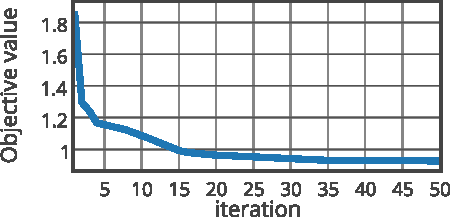
\includegraphics[width=0.6\linewidth]{./fig/objective_function_walk.pdf}
		\caption{Experiment 1: Evolution of the cost function along the iterations.}
		\label{fig:objective_walk}
\end{figure}
The overall movement is depicted in Fig.~\ref{fig:moviepicture} (see also the accompanying video). The steps are very large for the humanoid robot (which is $1.60\,$m tall).

Fig. \ref{fig:zmp_walk} shows the ZMP trajectory on the Y axis resulting from the OCP, compared to the estimation coming from force sensors measurement. The ZMP is very similar to what could be obtained by a classical WPG with assumption of flat contact. The proper tracking on the real robot shows the dynamic consistency of the output of the OCP.

\begin{figure}[!ht]
	\centering
	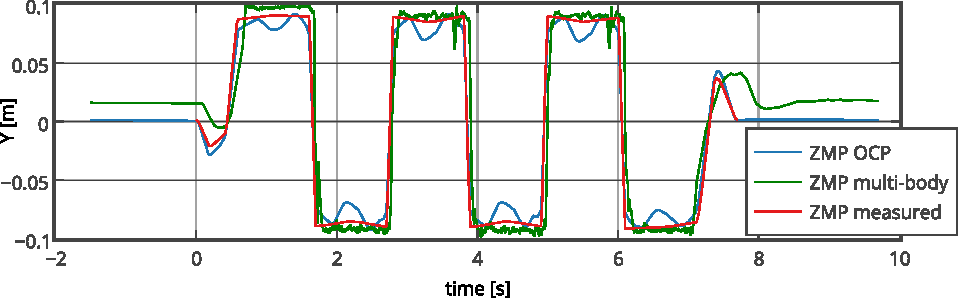
\includegraphics[width=1\linewidth]{./fig/zmp-walk-45cm.pdf}
		\caption{Experiment 1: ZMP trajectories obtained from the OCP, the multi-body dynamics and the measurements.}
		\label{fig:zmp_walk}
\end{figure}



\begin{figure*}[!ht]
  \begin{center}
  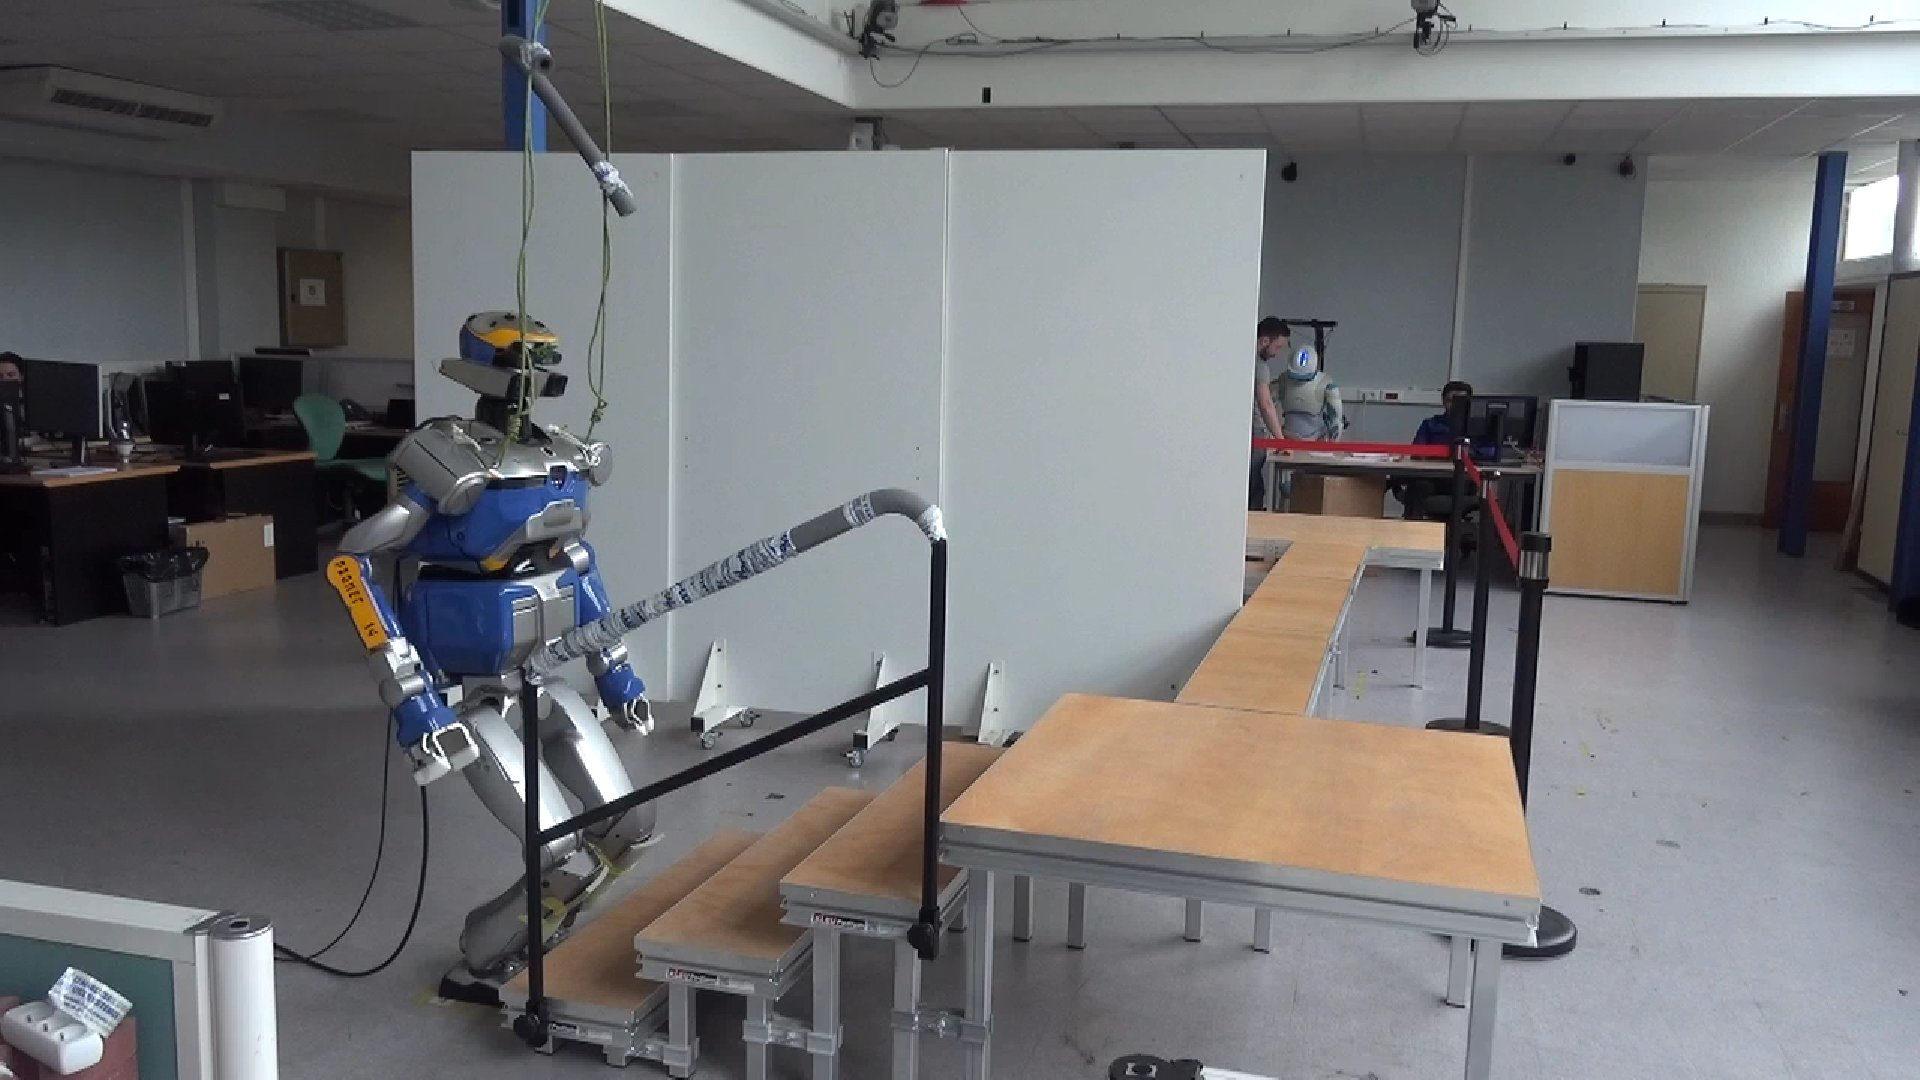
\includegraphics[trim={7.0cm 0.0cm 20.0cm 0.0cm}, clip, width=0.2\widthValue]
    {./fig/stairclimbing1.jpeg}
  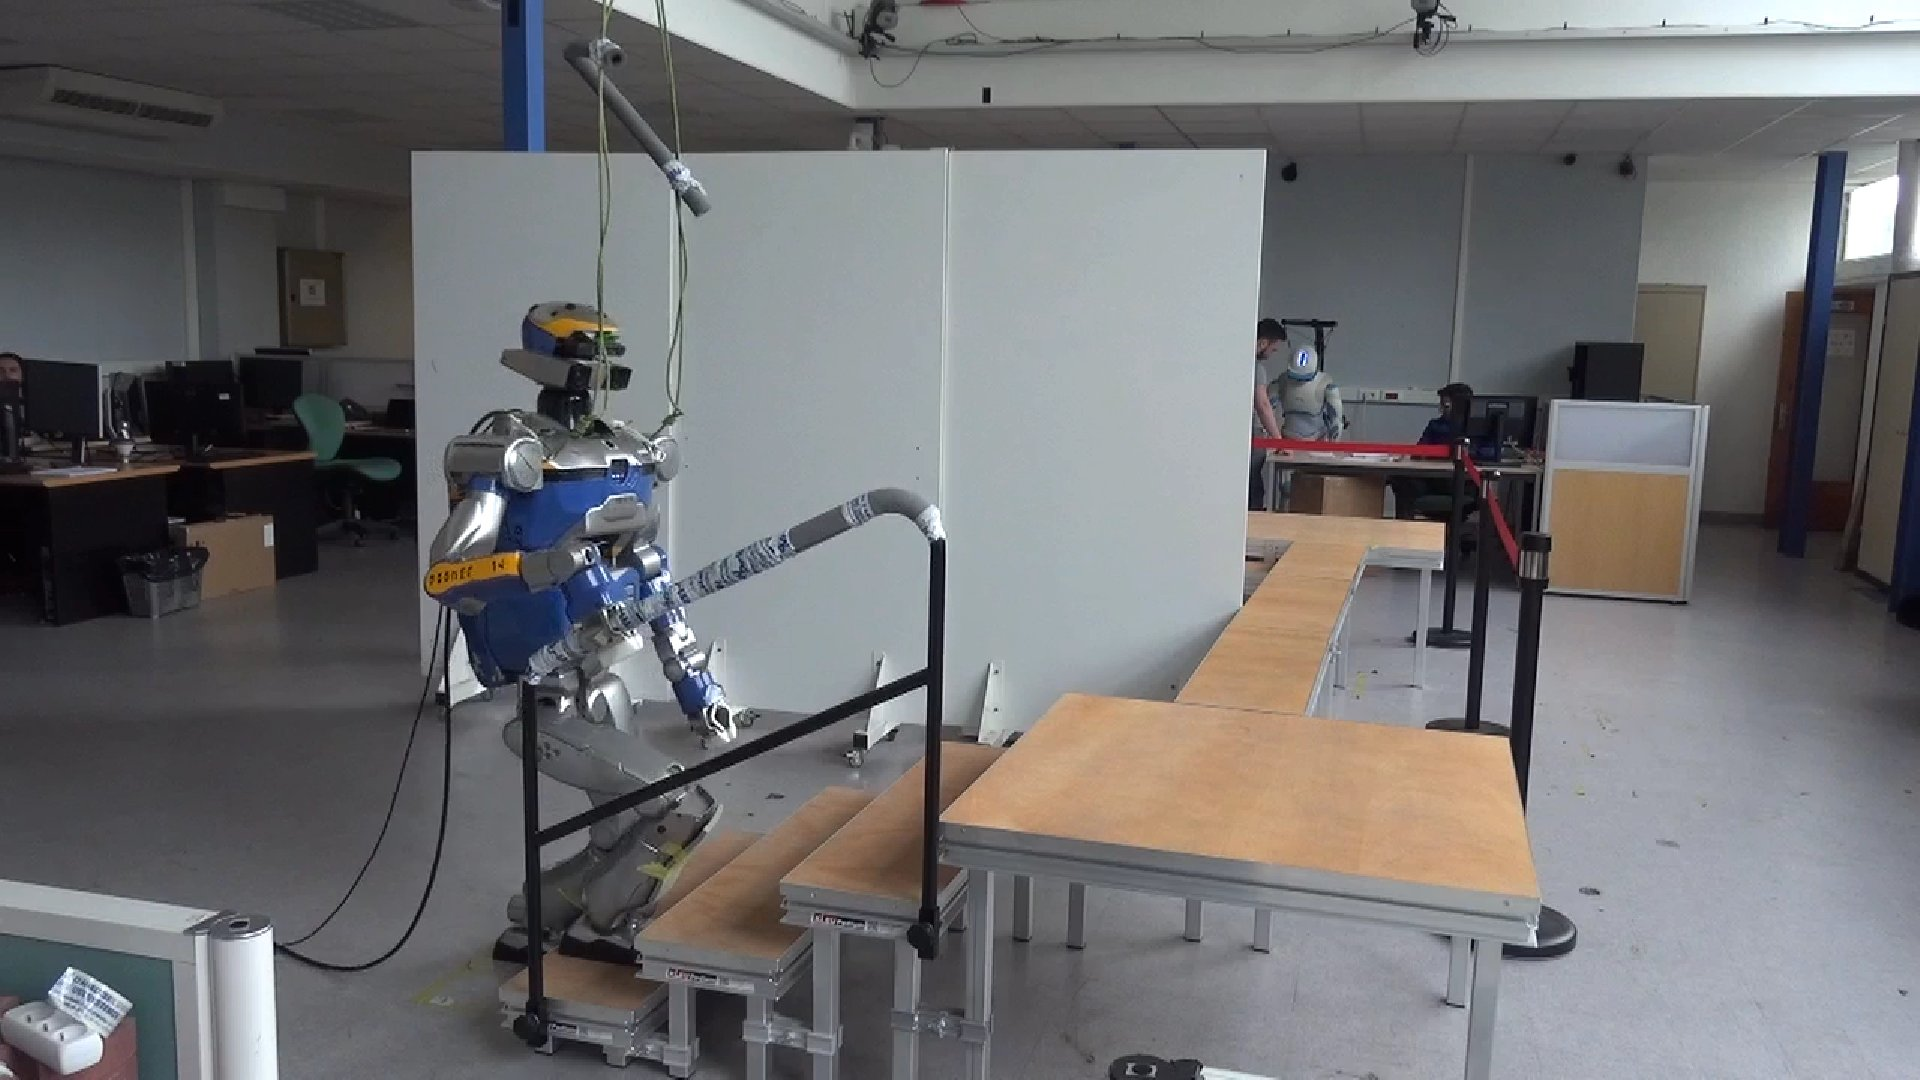
\includegraphics[trim={7.0cm 0.0cm 20.0cm 0.0cm}, clip, width=0.2\widthValue]
    {./fig/stairclimbing2.jpeg}
  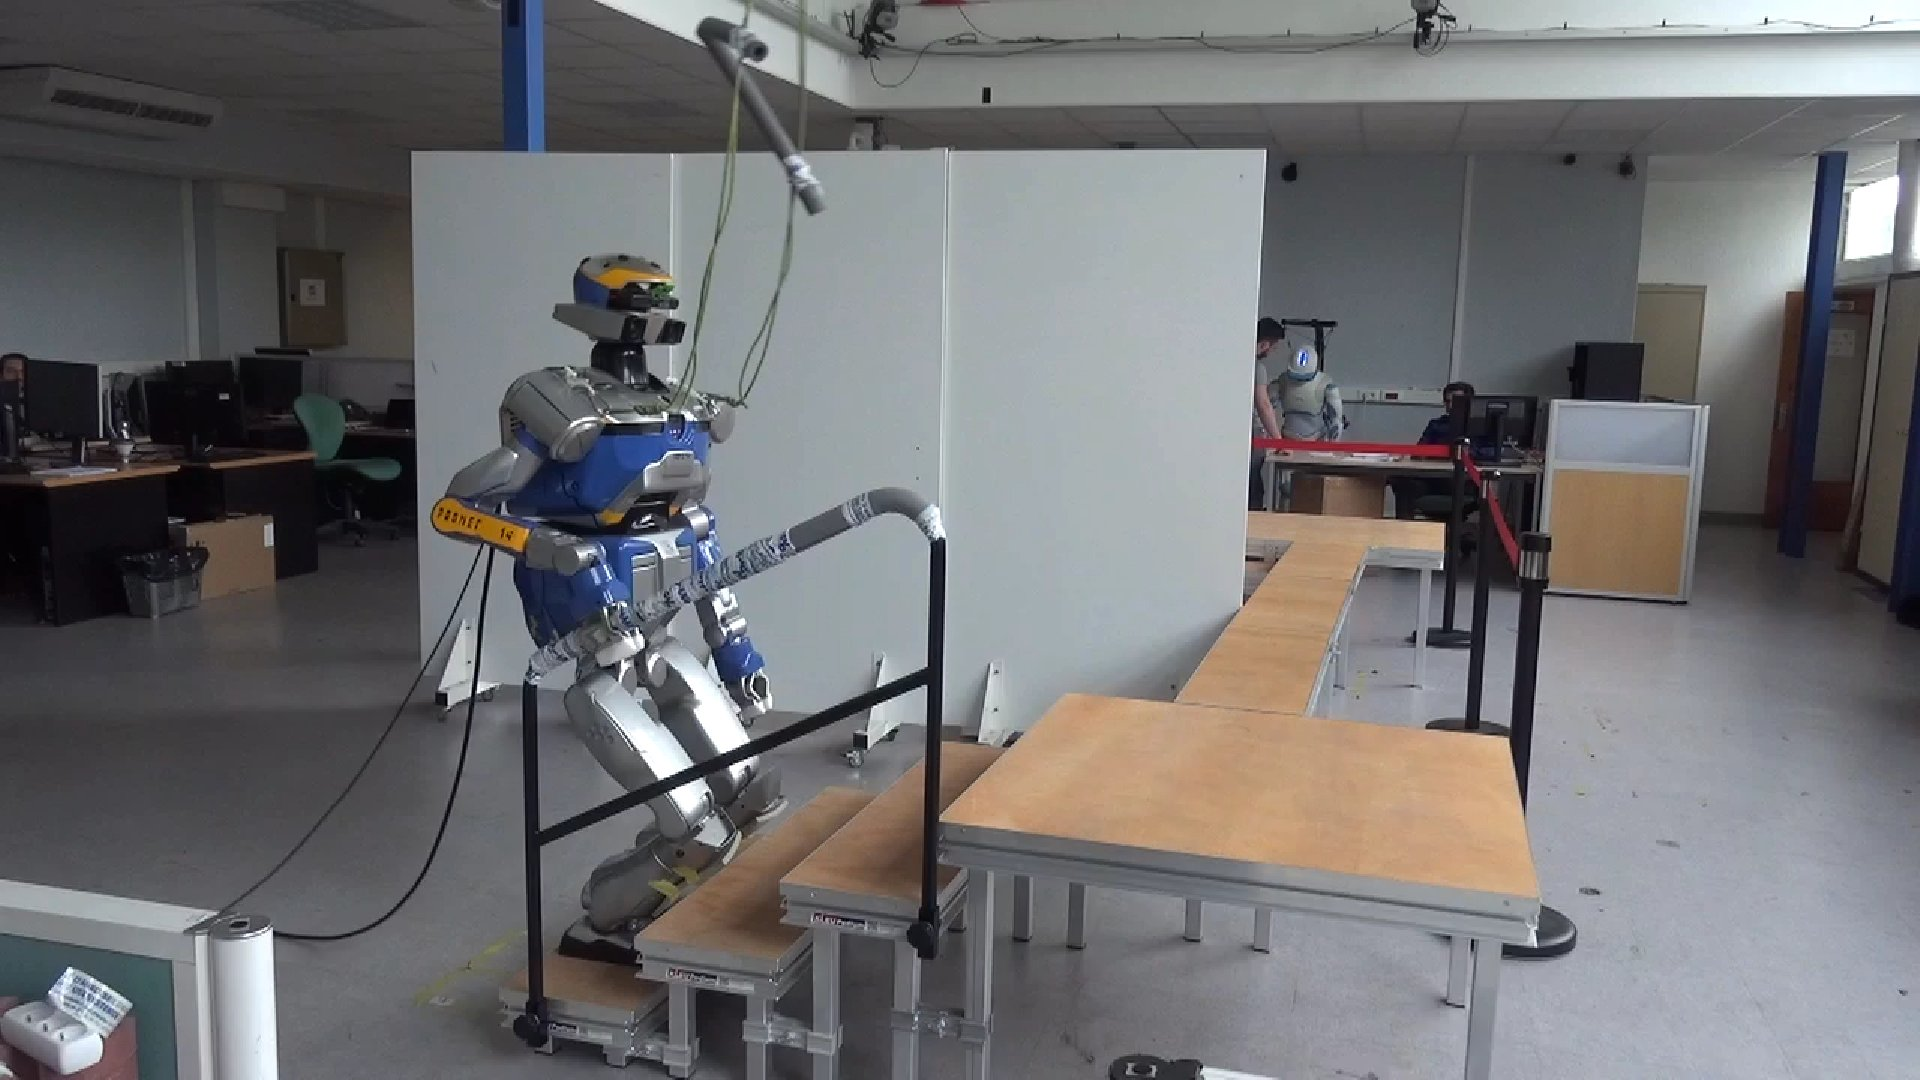
\includegraphics[trim={7.0cm 0.0cm 20.0cm 0.0cm}, clip, width=0.2\widthValue]
    {./fig/stairclimbing3.jpeg}
  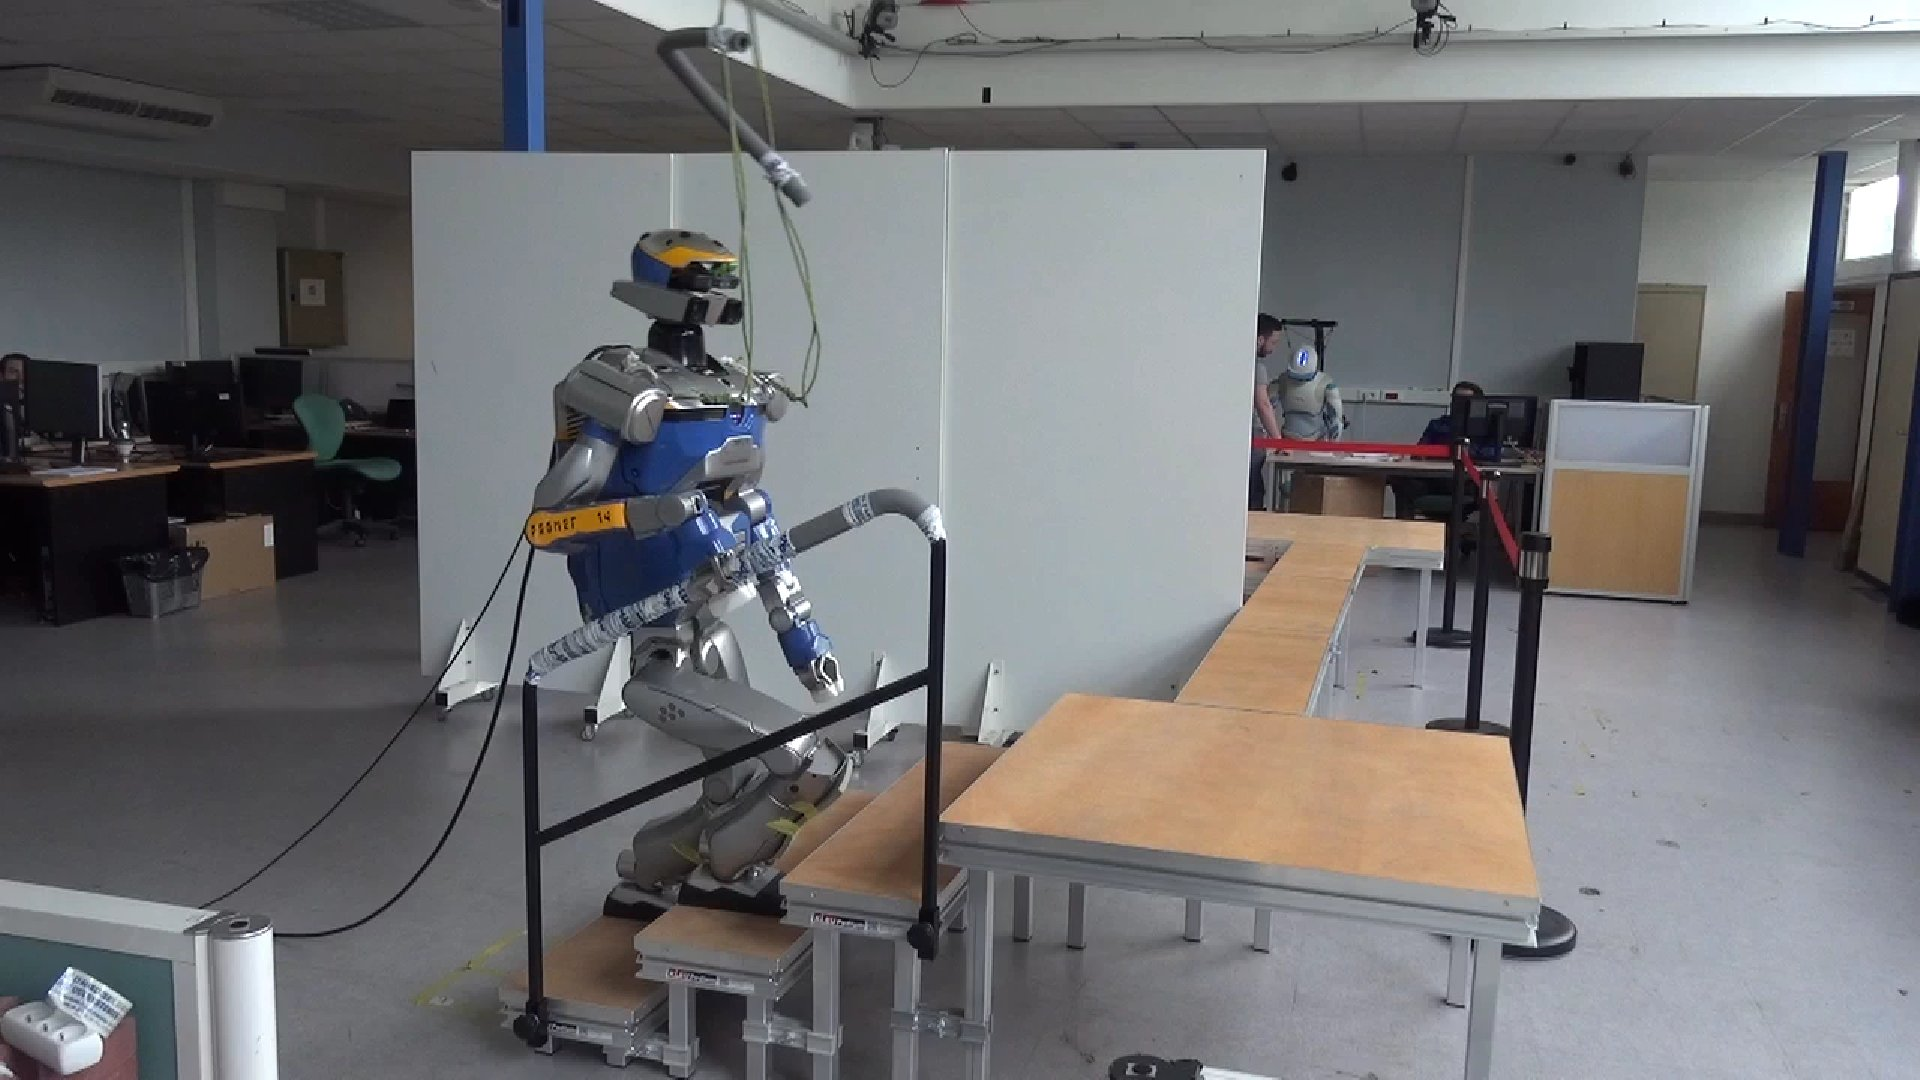
\includegraphics[trim={7.0cm 0.0cm 20.0cm 0.0cm}, clip, width=0.2\widthValue]
    {./fig/stairclimbing4.jpeg}
  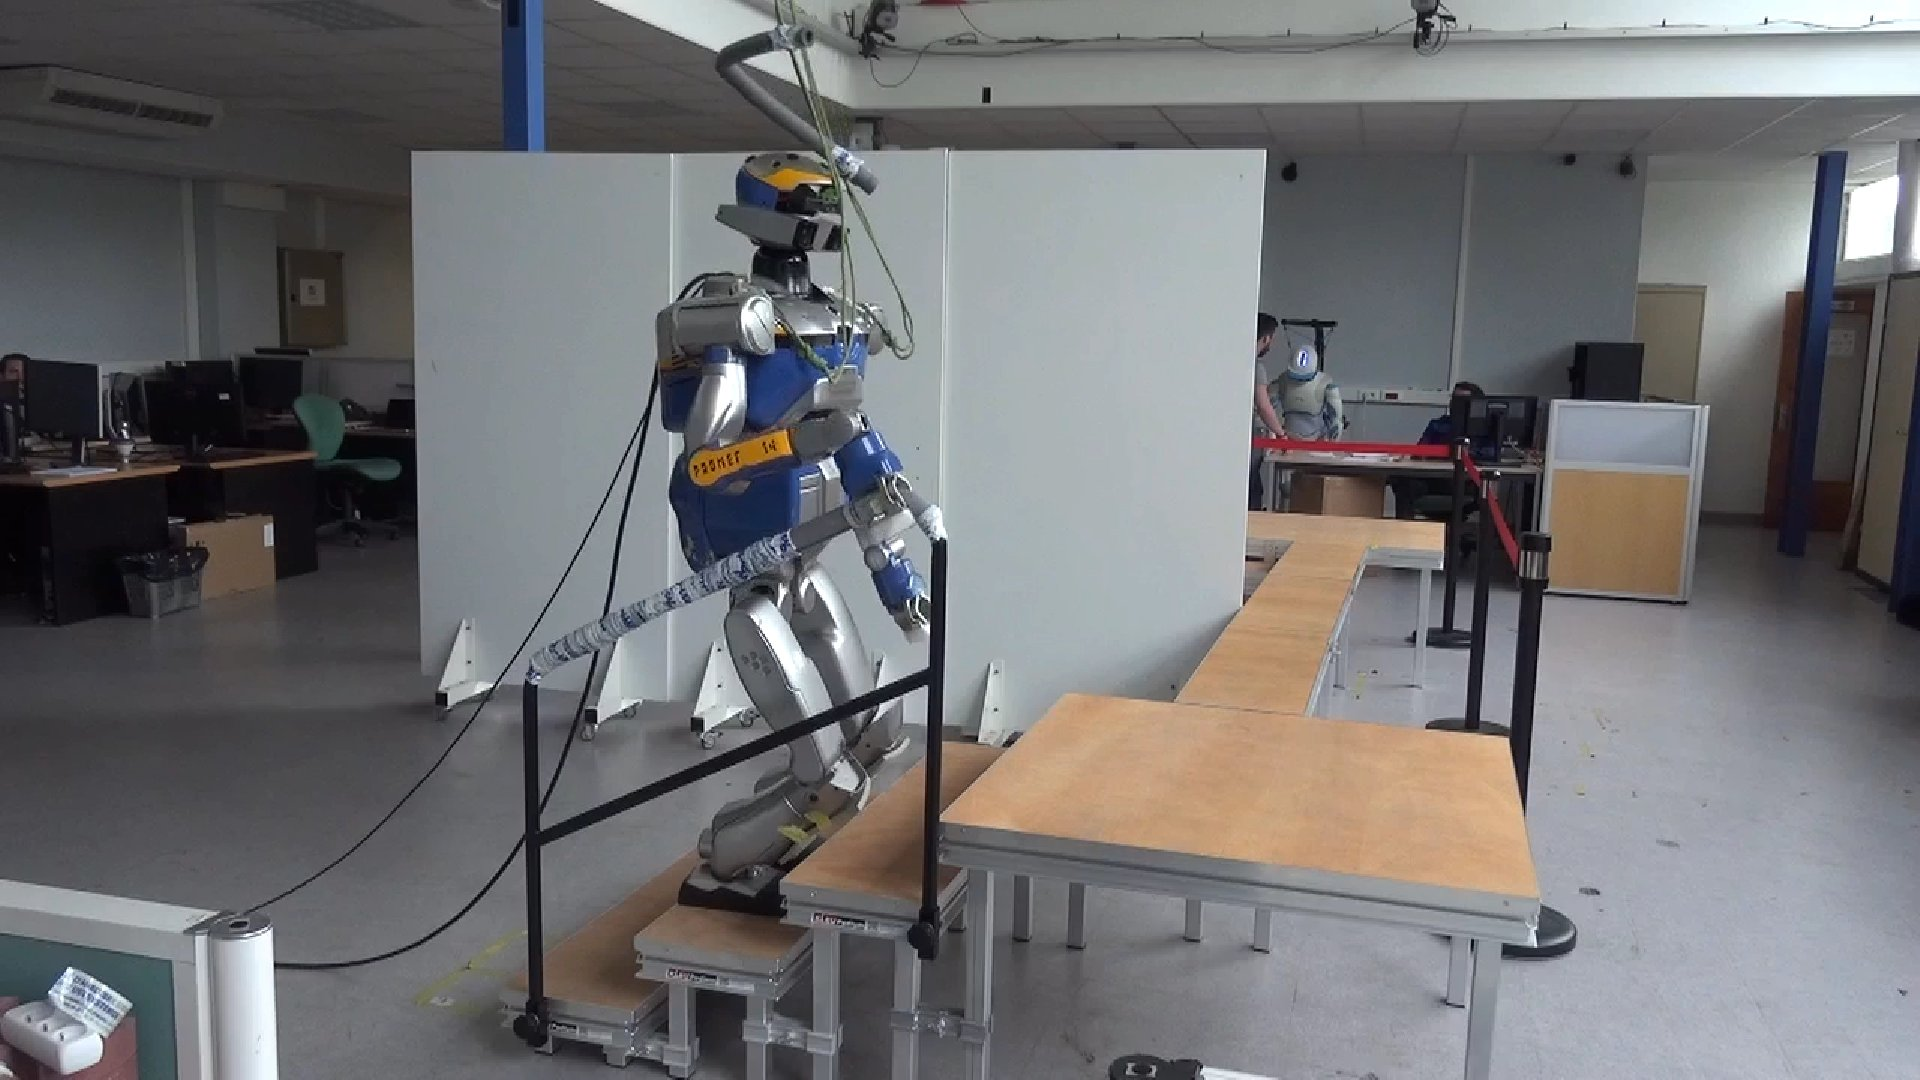
\includegraphics[trim={7.0cm 0.0cm 20.0cm 0.0cm}, clip, width=0.2\widthValue]
    {./fig/stairclimbing5.jpeg}
  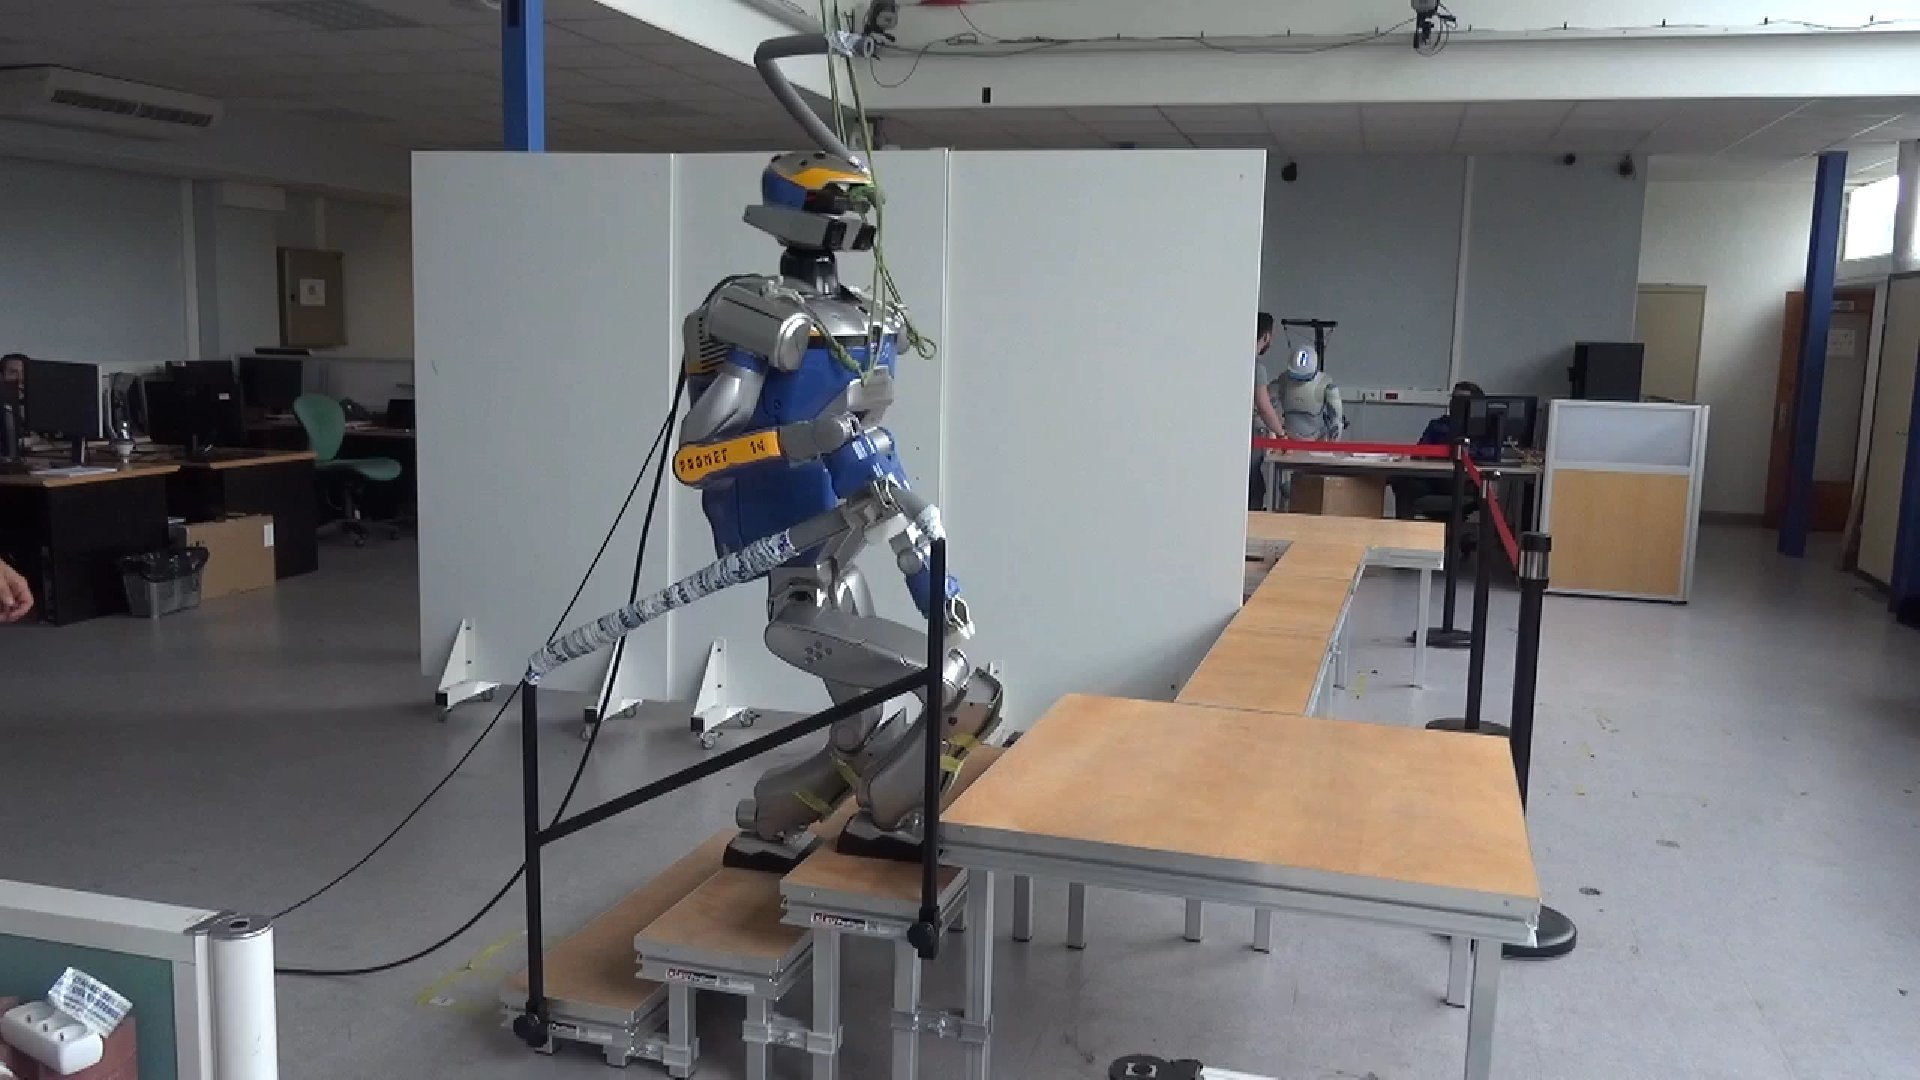
\includegraphics[trim={7.0cm 0.0cm 20.0cm 0.0cm}, clip, width=0.2\widthValue]
    {./fig/stairclimbing6.jpeg}
  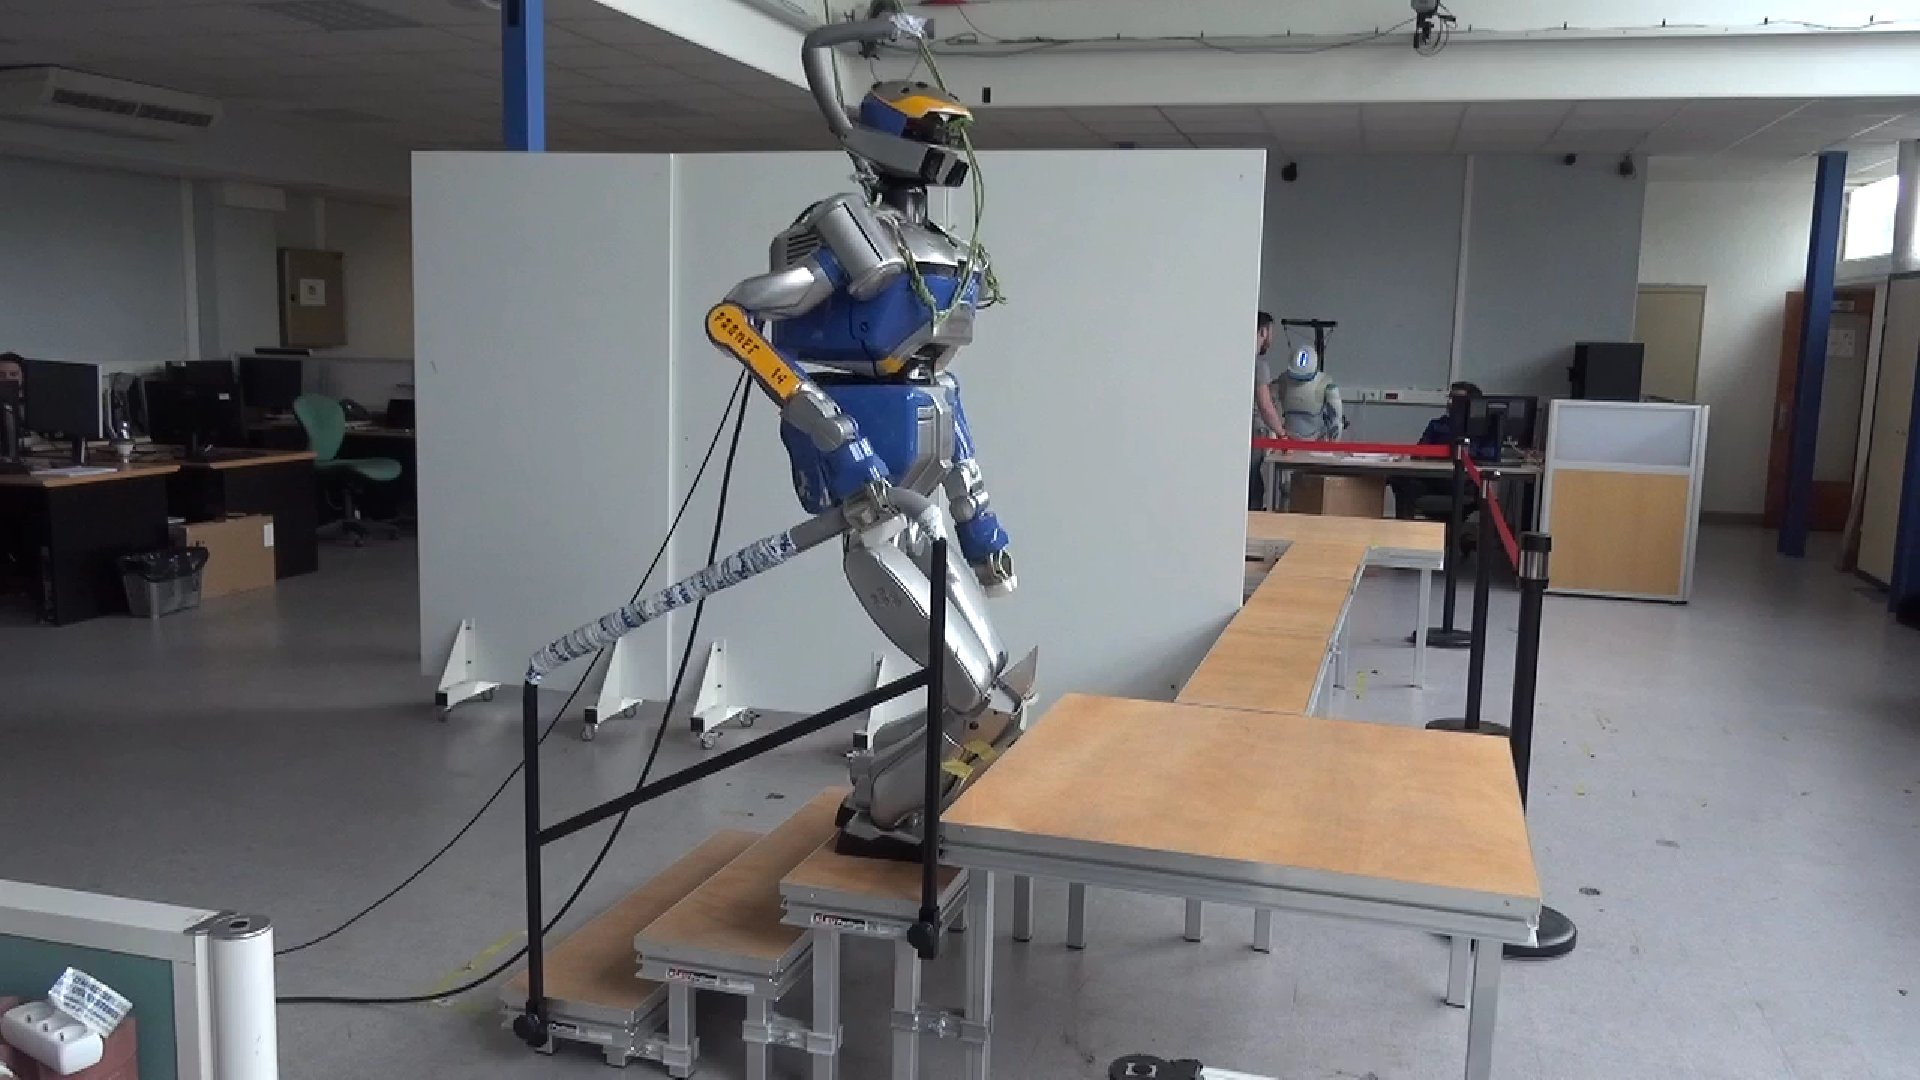
\includegraphics[trim={7.0cm 0.0cm 20.0cm 0.0cm}, clip, width=0.2\widthValue]
    {./fig/stairclimbing7.jpeg}
    %trim={<left> <lower> <right> <upper>}
  \caption{
   Experiment 2: Climbing the stairs of $15$cm height while using the handrail.
  }
  \label{fig:moviepicture2}
  \end{center}
\end{figure*}

\subsection{Experiment 2: Climbing stairs equipped with a handrail}

In the climbing scenario, the contact sequence given by the planner is no more cyclic and takes around $1$s to be computed. The computation of a feasible trajectory to climb one stair is done in less than $5.5$s after $85$ iterations. 

Fig. \ref{fig:foot_forces} illustrates both the forces computed by the solver and the forces exerted on the real robot. The simulated and measured forces do not match exactly but they have similar variations. In both cases, we observe that the robot makes use of its right hand either for pulling or pushing. The oscillations in the forces response are mainly due to the presence of a flexibility part in the robot's feet and to the compliance of the handrail. These two physical disturbances are not considered in our framework.

\begin{figure}[!ht]
	\centering
	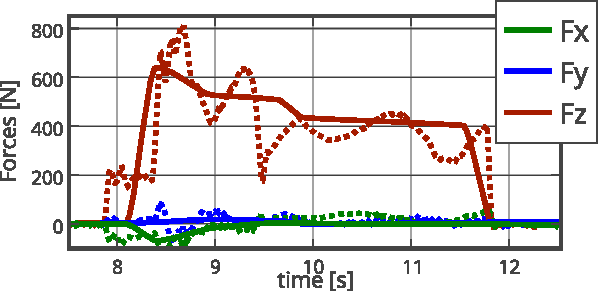
\includegraphics[width=0.9\linewidth]{./fig/Right_Foot_Forces.pdf}
	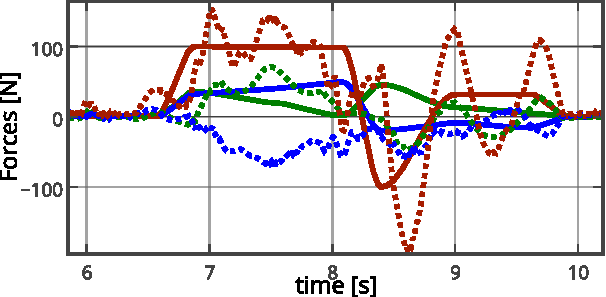
\includegraphics[width=0.85\linewidth]{./fig/Right_Hand_Forces.pdf}
		\caption{Experiment 2: Reference (solid line) and measured (doted line) forces at the right foot (on top) and hand (on bottom) during one contact phase. The reference forces are properly tracked (even if some flexibility can be observed).}
		\label{fig:foot_forces}
\end{figure}

\begin{figure}[!ht]
	\centering
	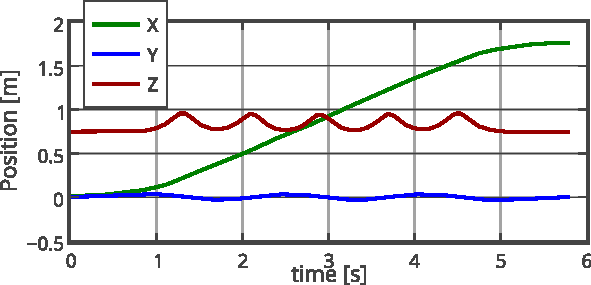
\includegraphics[width=0.8\linewidth]{./fig/running_traj.pdf}
		\caption{Experiment 3: COM trajectory for the running scenario. One can recognize the ballistic shape of the Z component.}
		\label{fig:running}
\end{figure}

\subsection{Other motion}

\begin{figure}[!ht]
  \begin{center}
   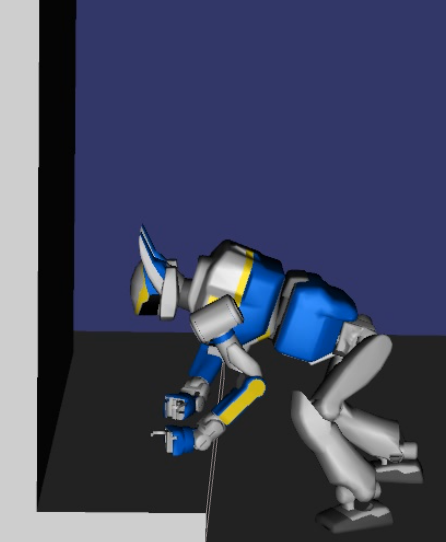
\includegraphics[clip, width=0.24\linewidth]{./fig/stand1.png}
  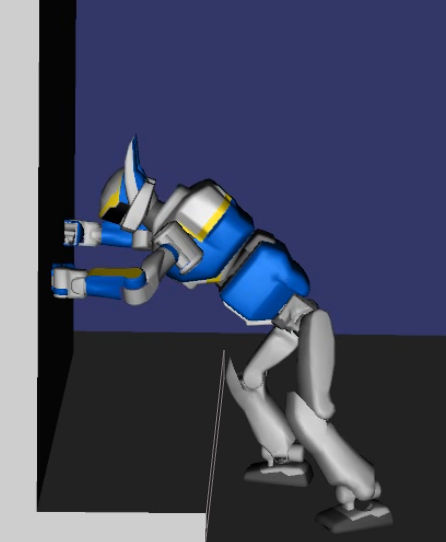
\includegraphics[clip, width=0.24\linewidth]{./fig/stand3.png}
  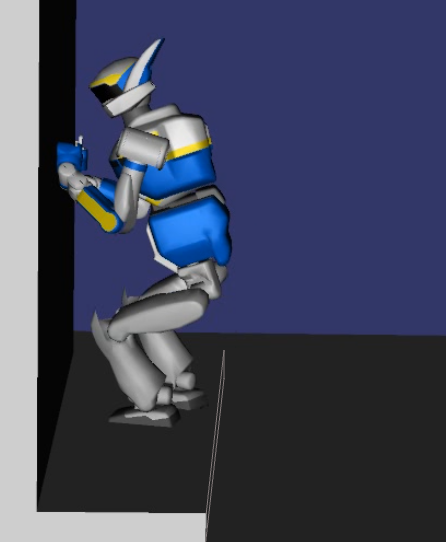
\includegraphics[clip, width=0.24\linewidth]{./fig/stand4.png}
  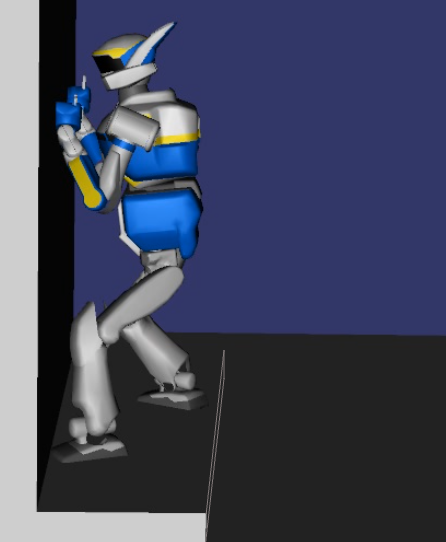
\includegraphics[clip, width=0.24\linewidth]{./fig/stand5.png}
  \caption{Experiment 3: The robot is standing up helped by the contacts which it is making with the surrounding environment.  }
  \label{fig:standing}
  \end{center}
\end{figure}

We also report two movements in simulation to exhibit some additional aspect of the approach. 
A running movement was computed with a periodic contact sequence. It implies some ballistic phases that the solver properly manages to handle. The resulting COM trajectory is presented in Fig.~\ref{fig:running}.

A standing-up motion was planned, where the robot exploits the proximal environment in order to stand up. For this movement, the sequence of contact configurations is nontrivial and would have been difficult to manually build. This motion is illustrated by Fig. \ref{fig:standing}.
See also the companion video.
